\chapter{Technical Details}
\label{chap:implementation}

\section{Virtualization}
The most important concept of cloud computing and therefore also for IaaS systems is virtualization. Nowadays every cloud computing system is virtualized. This means that all the user's cloud computing applications run in virtual machines. In the case of IaaS systems the user buys a VM and can install whatever system he likes on it \cite{Arzuaga_2010}. 

Virtualization brings many advantages. A lot of crucial concepts of cloud computing are a lot easier with virtualized systems. On example is load balancing: Virtual machines can be copied and can be migrated on other physical machines without any problems - Figure \ref{fig:virtualization_live_migration} illustrates this graphically. The following section will give you a greater insight into load balancing strategies \cite{Arzuaga_2010}.

\begin{figure}
	\centering
		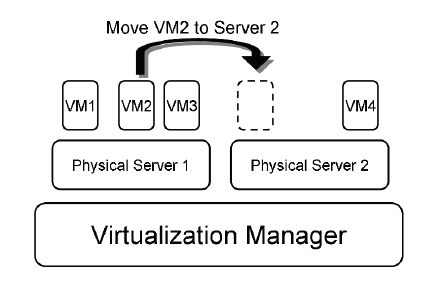
\includegraphics{virtualization}
	\caption{Virtualization and Live VM Migration in Cloud Computing Systems \cite{Arzuaga_2010}}
	\label{fig:virtualization_live_migration}
\end{figure}

\section{Load Balancing}
\label{sec:load_balancing}
As mentioned in the previous section, the applications on cloud computing systems run in virtual machines, and these VMs run in physical machines. Furthermore, there is a huge variation on the load (or resource needs) on the applications, therefore if there run too many applications (or VMs) on one physical machine it may get overloaded. This is why one needs load balancing. Load balancing should avoid that the physical machines have to handle more resources than they can offer. These resources can be CPU, RAM or storage space. If there run too many VMs on one physical machine this can mean a tremendous slow down of the VMs running on it. But slow VMs and applications are not the only problems, that bad load balancing would cause. If a application does not have sufficient resources, often the Service Level Agreement (SLA) is violated. A SLA is the agreement between customer and provider that guarantees certain parameters like performance and availability. A violation can mean that the cloud computing provider may have to give discount because of the violation or the customer decides to change to another cloud computing provider. As you can see good load balancing is crucial in the field of cloud computing \cite{Chen_2014}. 

\subsection{Load Balancing Algorithms}
There are many approaches on how load balancing algorithms should work, but they all have something in common: the input and the output. Every algorithm has to watch over the states of the physical and virtual machines and has to decide if a VM gets moved from. Furthermore, it has to decide which VM has to be migrated to which physical machine \cite{Chen_2014}.

Many common load balancing algorithms are based on the current states of the PMs and VMs. They therefore are called "reactive" algorithms. This means that when the resource utilization on a certain PM reaches a certain threshold, a VM gets migrated to another PM. This algorithm is rather easy to implement, as it only has to watch the current resource utilization at the physical machines, but the disadvantages are that it only considers the current state of the system and that when a the threshold is reached most often, an imbalance situation is yet the case. Furthermore, it cannot guarantee a long-term balance situation, as it only acts on the parameters known at that point of time \cite{Arzuaga_2010,Chen_2014}.

Other algorithms are based on a "proactive" approach. In these algorithms the physical machines try to predict the resource demand of the VMs running on them and if in the near future there would be a overload they migrate a VM to another physical machine which predicts a lower resource utilization. This has the advantage that if the algorithm works as desired and the estimates on the resource demands of the VMs are approximately correct, there won't be any more overloads, because the algorithm would predict correct and migrate the VMs before the physical machine is overloaded. Usually the proactive approaches give better results than the earlier discussed reactive approach. But, however, there are also disadvantages. The first one is that the physical machine does under usual circumstances not know, which VM should be migrated to another PM. Furthermore, in the long run this approach also does not create a balanced state, because it only predicts a certain time span in the future. Finally, there have to be made a lot of calculations to predict the resource needs of the VMs (this is usually done by a Markov model), especially when there are a lot of VMs per physical machine. This often creates a big load just for the load balancing algorithm \cite{Beloglazov_2013,Chen_2014}.

\section{Resilience Planning}
As customers in nowadays IT world expect applications to be accessible anytime, anywhere from any device an "always-on, always-available" service is pervasive. As with every technical product also parts of an cloud infrastructure can experience several failures and to provide high availability it is essential to consider resilience when operating services in the cloud \cite{IBM_2014}. Data and it's volume to be managed is getting more complex  and made high-availability solutions and disaster recovery strategies mandatory. 

An important point is to address the evolvements and advances brought by the cloud in the resilience planning process. In contrast to dedicated hardware or single physical servers, IaaS provides heavy virtualization of physical compute resources which can be put together in a single software-based virtual network. Due to this reasons the possibility for failures, especially on the software side, has increased and it's clear that errors will occur \cite{IBM_2014}.   
There are two metrics driving resilience:
\begin{itemize}
	\itemsep0em 
	\item Recovery Time Objective (RTO): This is basically the time it takes to restore a service after it has experienced a failure.
	\item Recover Point Objective (RPO): This is an indicator for the data los after a failure.
\end{itemize}

To make an IaaS cloud infrastructure resilient geographic distribution of data centres connected via WAN plays an important role. On the one hand latency can be decreased due to the smaller distance between an edge location providing the service and the end-user requesting it and on the other hand geographic spreading adds redundancy because the same service can be provided from another data centre possibly being thousands of kilometres away from the affected one. 
During resilience planning you first have to identify which risks you want to consider and how to set the constraints for your service level agreement. These results are the basis for modeling the infrastructure distribution. Important tasks are investigating the underlying network and connections to identify so called shared risk groups (SRGs) which suffer in case of a specific failure. With this knowledge you can decide which mechanisms should be taken. Before any recovery can be started, failures have to be detected which by periodic heartbeats or network alarms of infrastructure components. After that a healthy component starts running the affected service and traffic must be redirected via networking reconfiguration subsequently to prevent further requests to the unhealthy instance \cite{Resilience_2014}. How these backup strategies can look like will be explained in more detail in the following section. 

\section{Backup Strategies}
A backup is a copy of important files and is usually made to reduce the chance of data-loss.

Backups don't have a high priority for the average user and most of them don't even back up their data 
\cite{stat_backup} but the loss of data is very costly and time-intensive if you don't take precautions in form of a backup.

One Backup strategy would be the „3-2-1 rule“ which is widely known. It describes a basic and simple strategy and avoids a single point of failure.
The following principles are the core strategy:
\begin{itemize}
	\itemsep0em 
	\item Have at least three copies of data
	\item In two different formats
	\item with one of those copies off-site
\end{itemize}
The three copies are including the one you already use, so you would have 2 backups, stored on 2 different media types (e.g. hard drive and DVD) in a different format and one of these have to be off-site. That means it should be stored somewhere else than the other copy (e.g. Out of the house).

This prevents single point of failure: When one hard drive is damaged, you have a second copy. If the format is corrupted, you have another backup in a different format. If something happens to the location, you have one backup off-site, since one event can't destroy both copies.
This strategy doesn't prevent data-loss, but it prevents most of the cases \cite{micro_2013}.
IaaS comes here into play in multiple parts: You can store backups online to have them off-site. You don't have to buy extra hardware and store them somewhere else. You can store your backups on different cloud providers to prevent data-loss with one. Many cloud providers offer software to automatically backup your data to their cloud so there is less work for the user in that regard. In addition, cloud providers have big datacenters and have measures against data-loss, so it is safer to store one copy there \cite{google_centers}.


\section{Monitoring}
Monitoring is an essential part for deployed systems for both,  dedicated hardware structures and cloud computing systems. It enables to discover and analyze failure, bad configuration, performance bottle necks and many other issues that are important parts of software maintenance. Cloud computing systems are made to be highly scaleable and elastic. But these two characteristics make it hard to monitor cloud computing systems as monitoring of high scaling systems requires to collect, store and analyze a lot of data in real time, which can be computationally highly expensive. Furthermore, the high elasticity shows an extra challenge, as the whole environment can change in a very short period of time in modern clouds \cite{Ward_2014}.

\subsection{Common Architectures for Distributed Systems}
\label{sec:common_arc_ds}
The most important architectures that are typical for monitoring distributed systems are:

\begin{itemize}
	\item Flat Pull Model: A central server polls all the machines he should monitor according to a schedule when machines join and leave.
	\item Hierarchical Pull Model: Monitoring servers poll a subset of all the servers which should be monitored. A central server then polls the monitoring servers.
	\item Hierarchical Push Model: The server themselves push information to a monitoring server which is assigned to them and the monitoring servers collect that information from their machines and push it to a central server \cite{Ward_2014}.
\end{itemize}

However, the just mentioned models for monitoring are modeled for grid and cluster computing. They are not always optimal for cloud computing systems as virtual machines can dynamically be added and removed and this creates the need for other approaches \cite{Ward_2014, He_2010}. 

\subsection{Architectures modeled for Cloud Computing}
In 2010, Huang \cite{He_2010} proposed a monitoring system he called "Push and Pull", which should combine the advantages of the push and pull. In current pull systems, the consumers (monitoring servers) pull information from the producers (virtual machines which should be monitored) in a certain interval. This approach is efficient but lacks in consistency. If the interval is too big, data is lost, but if the interval is too small it is inefficient as there is too much network traffic. In push systems on the other hand, producers tell the consumers changes whenever the changes are greater than a threshold. This can produce good performance depending on the threshold and all data changes are monitored, but if the threshold is too small, too much information is transmitted and this leads again to inefficiency. The Push and Pull model Huang suggests, should use both approaches in a mixed way depending on the situation. Therefore, Huang introduces a value called User Tolerant Degree (UTD). This value indicates if high accuracy is a core requirement for the user or if the user tolerates minor inaccuracy. In Push and Pull both approaches are used simultenously in different degrees. For example, if the UTD is small, the user won't tolerate inaccuracy and the push model will dominate over the pull model. This means that according to the UTD, the producer will push changes larger than a relatively small threshold to the consumer, but at the same time the consumer will pull with a long interval to be sure not to miss changes. But if the UTD is large (the user will tolerance inaccuracy), the pull model will dominate. The consumer will have a short interval in which he pulls information from the producer and the producer only pushes changes if they are bigger than a large threshold.

Another approach was proposed from Ward \cite{Ward_2014} in 2014. He called his system VARANUS and it is built up on a layered probabilistic multicast or gossip protocol. By dividing up computational complexity over the system, gossip protocols show great performance in large scale networks. Within the layers the peers communicate via push and pull with other peers which are nearby. The distance between peers is determined by measuring the round trip time between the peers. In VARANUS the communication is different from layer to layer. In the lower layers, there is a great bandwidth and therefore the exchange rate is high and the information is highly consistent, whereas in the higher layers, the information is sent in lower intervals, because else there would be a too high network traffic.
Figure \ref{fig:ward_varnus_architecture} shows the architecture of the VARANUS.
\begin{figure}
	\centering
		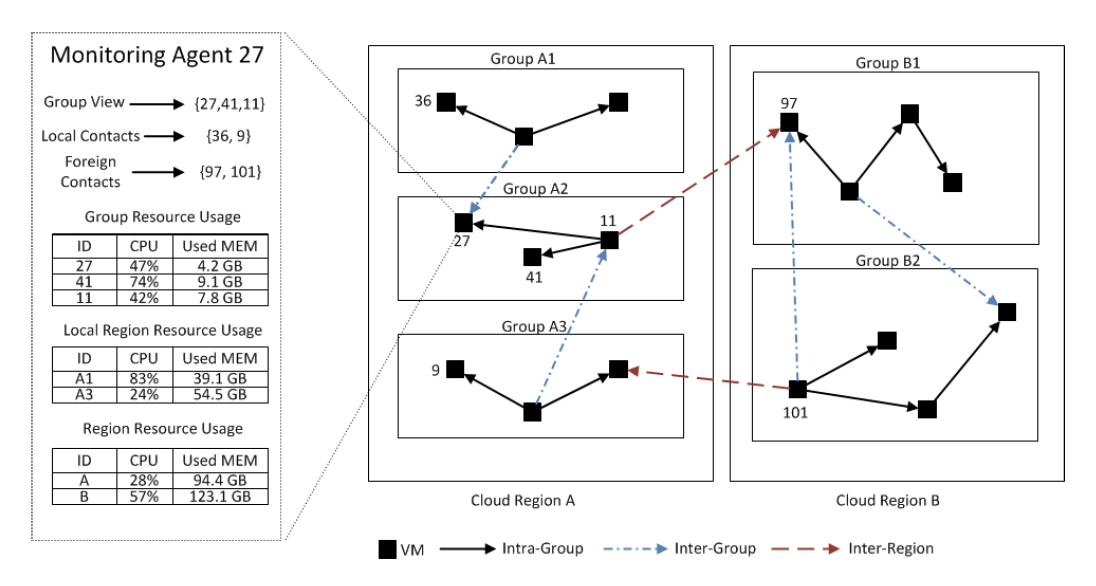
\includegraphics[width=\textwidth]{wang_monitoring}
	\caption{Architecture of the VARANUS monitoring system \cite{Ward_2014}}
	\label{fig:ward_varnus_architecture}
\end{figure}

Both architectures show significant improved results in terms of performance, latency and scalability in large scale deployment systems than the traditional systems for cluster and grid computing (discussed in section \ref{sec:common_arc_ds}).